\chapter{Chocolate Pudding Cake}
\label{ch:chocolatefridgecake}
\index{dessert}
\index{chocolate}
\index{cake}
\index{cookies}
\textit{Chocolate fridge cake with cookies}

Family member: Metzma Lucie \& Dan

\marginnote[20pt]{\\
    \textbf{Makes 1 cake} \\
    Prep time: 20 minutes + chill overnight in the fridge\\
    Cook time: 5 minutes \\
    \vspace*{\baselineskip}

     1 pack of Sheriff chocolate pudding \\
     1 pack of tea biscuits, Dare Traditions Social Tea brand \\
}

\newthought{Vasken} would eat half a pan of this.
\bigskip

\begin{enumerate}
    \item Follow the instructions on the chocolate pudding box.
    \item In a Pyrex or other baking dish, place tea biscuits to make a layer. You may need to break some cookies to cover all the bottom.
    \item While the pudding mixture is still hot, pour a thin layer on top of the cookies.
    \item Repeat layering cookies and pudding until desired height and finish with a layer of pudding at the very top.
    \item Refrigerate overnight.
\end{enumerate}

\begin{figure}
  \includegraphics[width=70mm]{dermardiros/images/Grandma fridge cake 1.jpg}
  \caption{Chocolate cake made by Dan}
  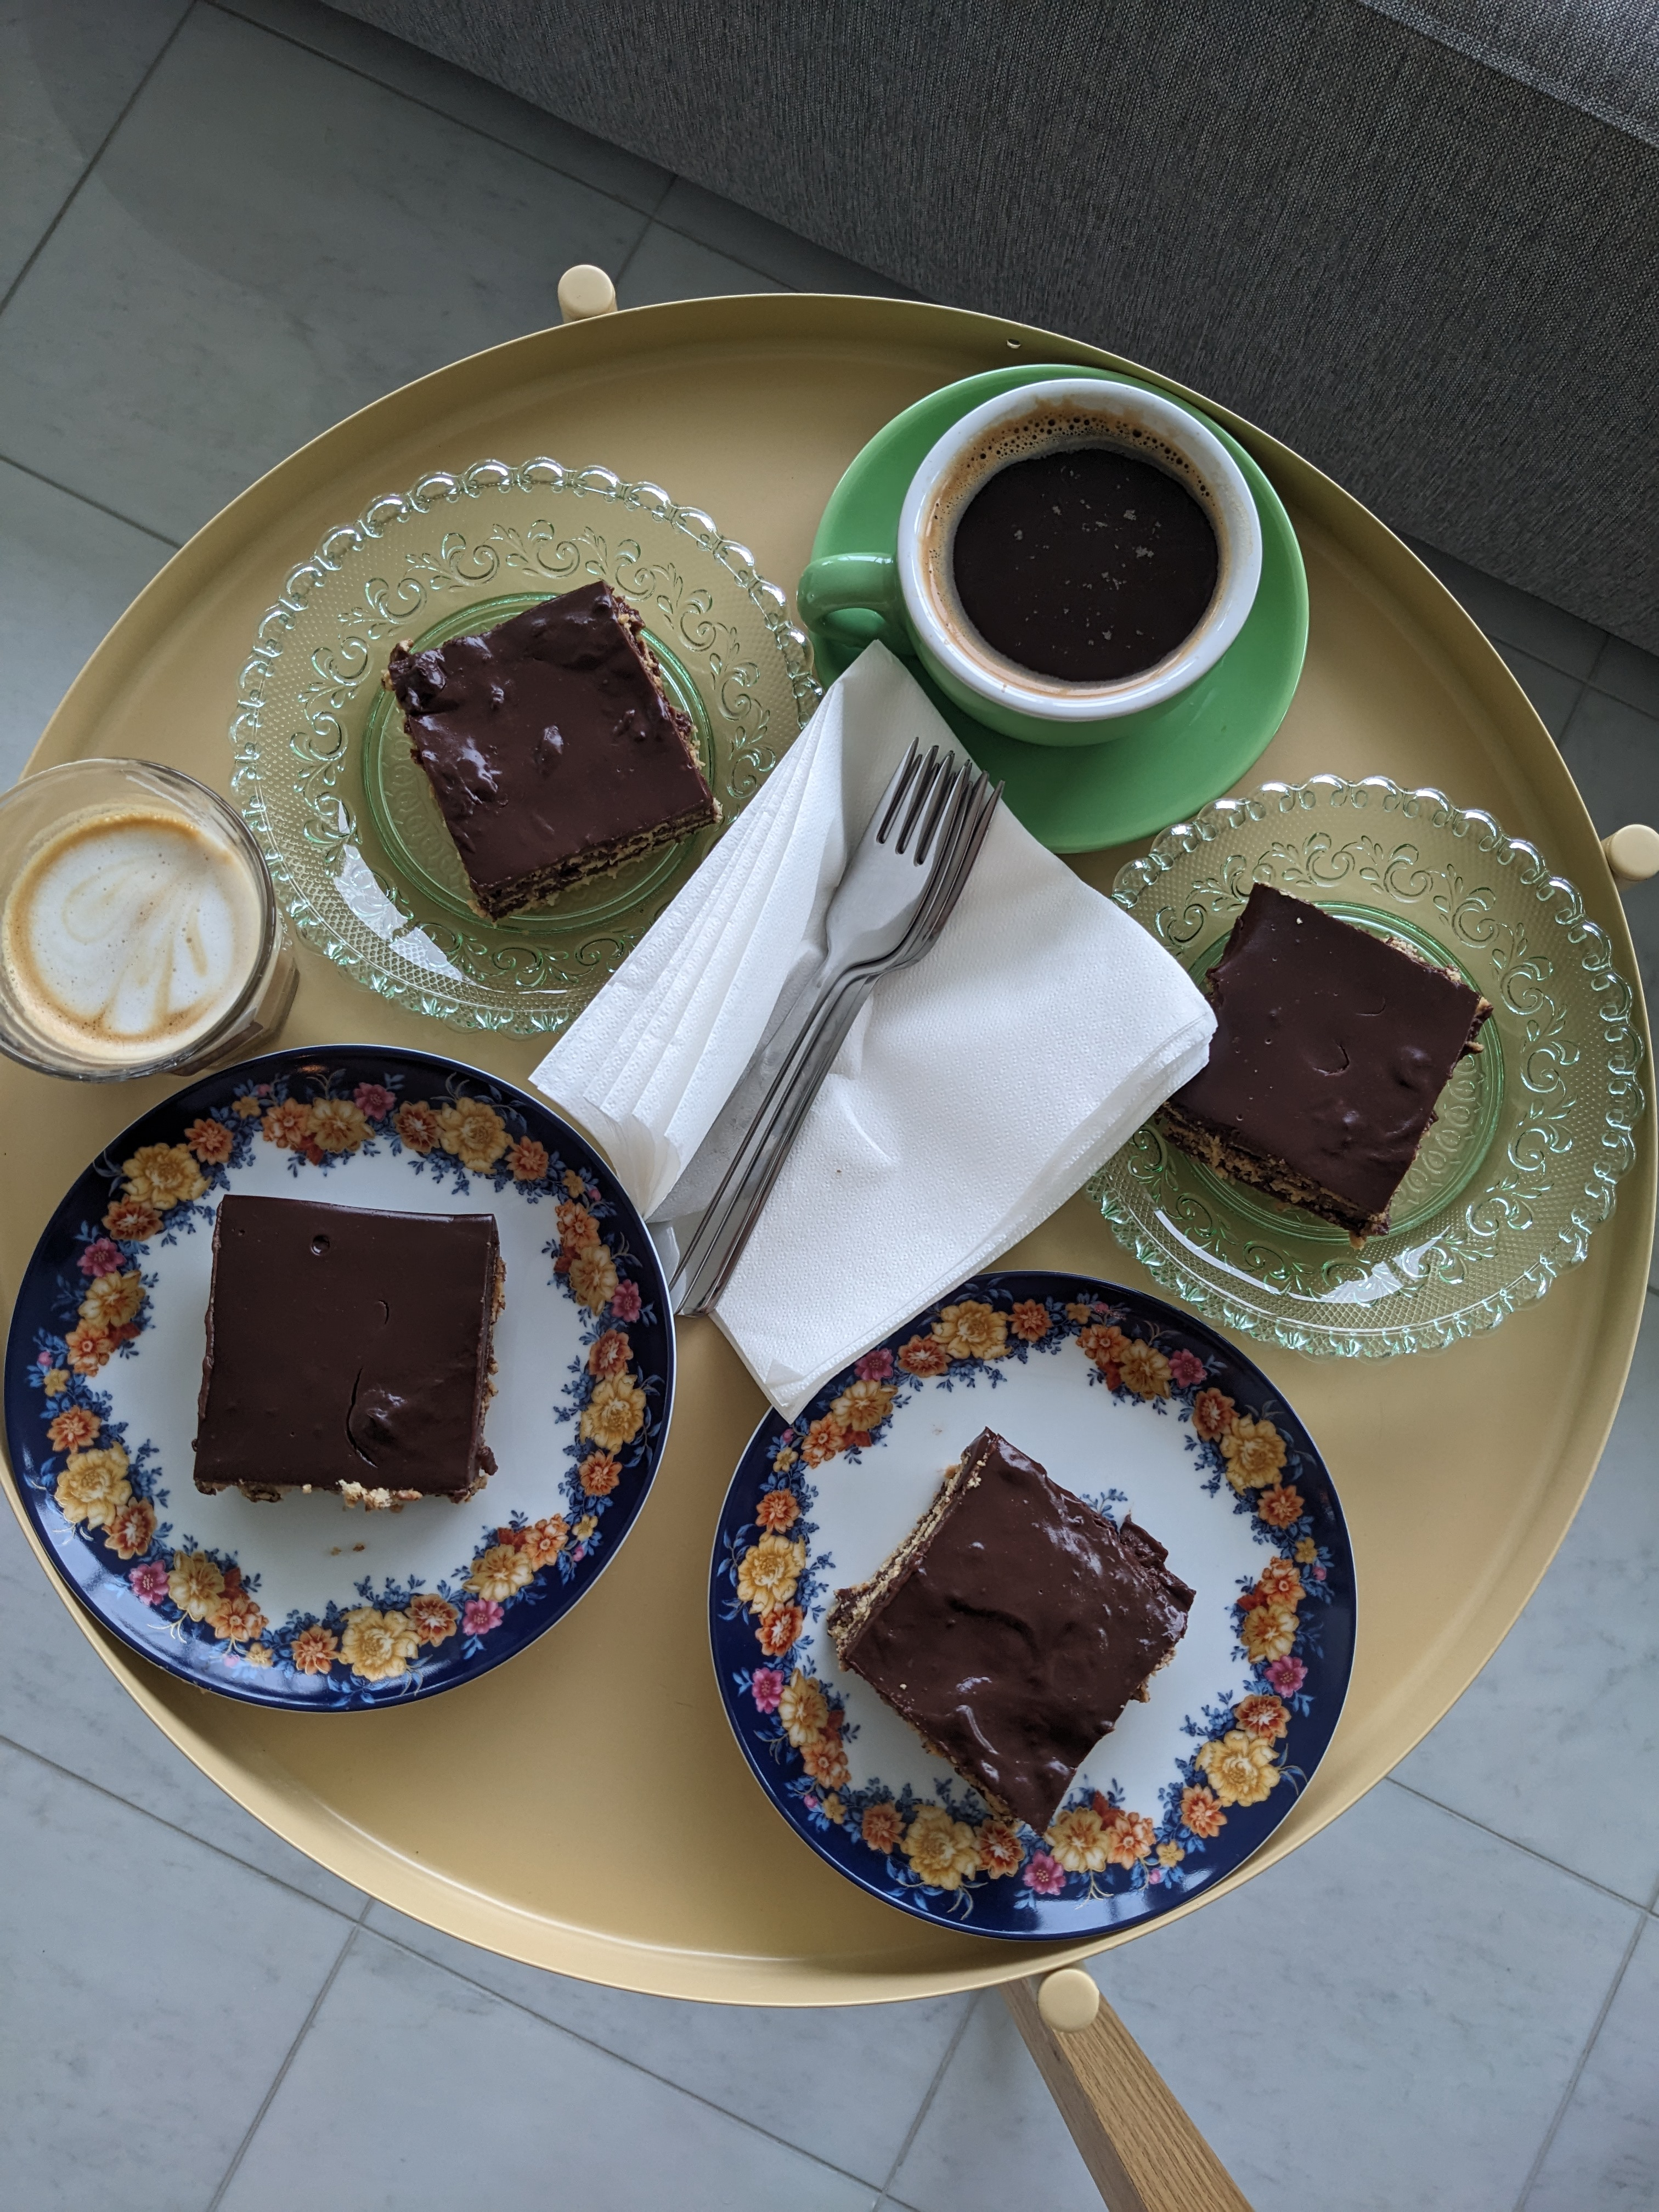
\includegraphics[width=70mm]{dermardiros/images/Grandma fridge cake 2.jpg}
  \caption{Coffee time at Dan's!}
\end{figure}